\documentclass[12pt]{article}

\usepackage{listings}
\usepackage{graphicx,url}
\usepackage[utf8]{inputenc}
\usepackage[brazil]{babel}

\title{Trabalho Teórico 5}
\author{Iyan Lucas Duarte Marques}
\begin{document}
\maketitle
\section{Exercícios Resolvidos}
\subsection{Exercício 1}
Mostre o somatório dos n primeiros números inteiros
\begin{figure}[ht]
    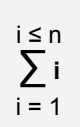
\includegraphics[width=50px]{1.png}
\end{figure}
\subsection{Exercício 2}
O Algoritmo de Seleção é uma solução conhecida para a ordenação
interna. Quantas comparações entre registros ele realiza?
\begin{figure}[ht]
    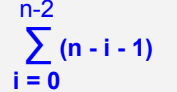
\includegraphics[width=4cm]{2.png}
\end{figure}
\subsection{Exercício 3}
b)
\subsection{Exercício 4}
(3 . 1) + (3 . 2) + (3 . 3) + (3 . 4) = 30
\subsection{Exercício 5}
(3 - (2 . 1)) + (3 - (2 . 2)) + (3 - (2 . 3)) + (3 - (2 . 4)) = -8
\subsection{Exercício 6}
2(1+2+3) + (x+x+x) = 12 + 3x
\subsection{Exercício 7}
5 . 4 . 0 = 0 + 0 + 6 + 12 + 12 + 0 = 30
\subsection{Exercício 8}
Sim, pois como os termos a0
, a1
e a5
são iguais a zero, o resultado dos dois somatórios é igual a (a2+ a3+ a4
)

\end{document}